\subsection{Standard ISO/IEC 15504}\label{15504}
Lo standard ISO/IEC 15504 descrive come i processi debbano essere continuamente controllati in modo da rilevare possibili rischi e debolezze che possano impedire il raggiungimento degli scopi prefissati e di individuarne le cause in modo di migliore l'efficienza dei processi. I risultati dei vari controlli devono essere oggettivi, ripetibili e comparabili perché possano essere utilizzati nel miglioramento dei processi.

\noindent Lo standard ISO/IEC 15504, conosciuto anche come SPICE(Software Process Improvement and Capability Determination), prevede per ogni processo un livello di capacità secondo la seguente ripartizione:

\begin{enumerate}[label*=\arabic*]
	\item \textbf{Incomplete process:} il processo non viene eseguito o non riesce a raggiungere i suoi risultati;
	
	\item \textbf{Performed:} il processo eseguito raggiunge i suoi risultati
		\begin{itemize}
			\item \textbf{Process performance attribute:} è la capacità di un processo di raggiungere gli obiettivi trasformando input identificabili in output identificabili.
		\end{itemize}
		
	\item \textbf{Managed process:} il processo viene eseguito in modo controllato in base a obiettivi definiti
		\begin{itemize}
			\item \textbf{Performance management attribute:} è la capacità del processo di elaborare un prodotto coerente con gli obiettivi fissati;
			\item \textbf{Work product management attribute:} è la capacità del processo di elaborare un prodotto documentato, controllato e verificato.
		\end{itemize}
		
		
	\item \textbf{Established process:} il processo viene eseguito basandosi su principi dell'ingegneria del software ed è in grado di raggiungere i risultati fissati
		\begin{itemize}
			\item \textbf{Process definition attribute:} l'esecuzione del processo si basa su standard di processo per raggiungere i propri obiettivi;
			\item \textbf{Process resource attribute:} è la capacità del processo di attingere a risorse tecniche e umane appropriate per essere attuato efficacemente.
		\end{itemize}
		
	\item \textbf{Predictable process:} il processo viene eseguito costantemente entro limiti definiti per raggiungere i risultati attesi
		\begin{itemize}
			\item\textbf{Measurement attribute:} sono gli obiettivi e le misure di prodotto e di processo vengono usati per garantire il raggiungimento dei traguardi definiti in supporto ai target aziendali;
			\item \textbf{Process control attribute:} il processo viene controllato tramite misure di prodotto e processo per effettuare correzioni migliorative al processo stesso.
		\end{itemize}
		
\item \textbf{Optimizing process:} il processo cambia e si adatta dinamicamente per raggiungere gli obiettivi aziendali
		\begin{itemize}
			\item \textbf{Process change attribute:} sono i cambiamenti strutturali, di gestione e di esecuzione vengono gestiti in modo controllato per raggiungere i risultati fissati;
			\item \textbf{Continuous improvement attribute:} sono le modifiche al processo sono identificate e implementate per garantire il miglioramento continuo nella realizzazione degli obiettivi di \gls{business} dell'organizzazione.
		\end{itemize}

\end{enumerate}

\noindent Ogni attributo di processo descritto sopra è misurabile e lo standard predispone 4 livelli diversi:
\begin{itemize}[label={}]
	\item \textbf{N} non posseduto (0\% - 15\%);
	\item \textbf{P} parzialmente posseduto (16\% - 50\%);
	\item \textbf{L} largamente posseduto (51\% - 85\%);
	\item \textbf{F} completamente posseduto (86\% - 100\%).
\end{itemize}

\subsection{Standard ISO/IEC 9126} \label{9126}
Con la sigla \textbf{ISO/IEC 9126} s'individua una serie di normative e linee guida preposte a descrivere un modello di qualità del software.
Esso divide i criteri qualitativi in 3 aree diverse:
\begin{itemize}

	\item \textbf{Qualità in uso:} rappresenta il punto di vista dell'utente sul software;
	\item \textbf{Qualità esterna:} misurano i comportamenti del software sulla base dei test, dall'operatività e dall'osservazione durante la sua esecuzione;
	\item \textbf{Qualità interna:} è la qualità del prodotto software vista dall'interno, si riferisce quindi alle caratteristiche d'implementazione quali l'architettura ed i codici sorgenti.
\end{itemize}

\noindent Il modello di qualità dello standard prevede 6 caratteristiche qualitative principali, suddivise in ulteriori sotto caratteristiche, misurabili quantitativamente tramite metriche specifiche.

\begin{figure}[h]
\centering
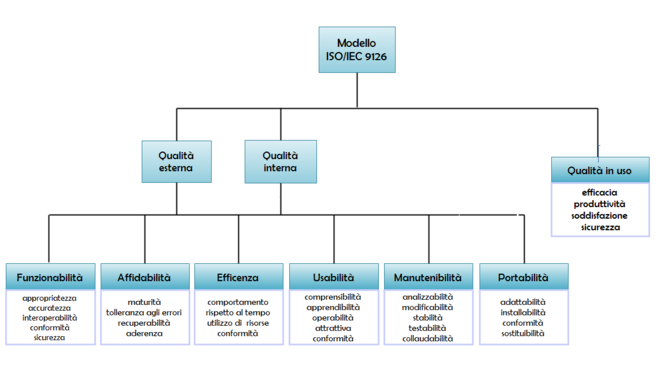
\includegraphics[width=0.7\linewidth]{img/ISO_IEC_9126}
\caption[Rappresentazione globale del modello ISO-IEC 9126]{Rappresentazione globale del modello ISO-IEC 9126}
\label{fig:ISO_IEC_9126}
\end{figure}


\begin{itemize}
\item \textbf{Funzionalità:} è la capacità di un prodotto software di fornire funzioni che soddisfano esigenze stabilite:

\begin{itemize}
	\item \textbf{Idoneità:}  rappresenta la capacità del prodotto software di fornire un appropriato insieme di funzioni per gli specificati compiti e obiettivi prefissati all'utente;
	\item \textbf{Accuratezza:} è la capacità del prodotto software di fornire i risultati concordati;
	\item \textbf{Interoperabilità:} è la capacità del prodotto software di interagire ed operare con uno o più sistemi;
	\item \textbf{Conformità:} è la capacità del prodotto software di aderire a standard, convenzioni e regolamentazioni;
	\item \textbf{Sicurezza:} è la capacità del prodotto software di proteggere informazioni e dati impedendo che persone o sistemi non autorizzati passano accedervi o modificarli.
\end{itemize}

\item \textbf{Affidabilità:} è la capacità del prodotto software di mantenere uno specificato livello di prestazioni:
\begin{itemize}
	\item \textbf{Maturità:} è la capacità di un prodotto software di evitare che si verificano errori o malfunzionamenti;
	\item \textbf{Tolleranza agli errori:} è la capacità di un prodotto software di mantenere un adeguato livello di prestazioni anche nel caso si verifichino errore o malfunzionamenti;
	\item \textbf{Recuperabilità:} è la capacità del prodotto software di ristabilire un adeguato livello di performance e di recuperare i dati interessati in caso di errori;
	\item \textbf{Aderenza:} è la capacità di aderire a standard, regole e convenzioni inerenti all'affidabilità.
\end{itemize}

\item \textbf{Efficienza:} è la capacità di fornire appropriate prestazioni relativamente alla quantità di risorse usate:
\begin{itemize}
	\item \textbf{Comportamento rispetto al tempo:} è la capacità di fornire adeguati tempi di risposta, elaborazione e velocità sotto determinate condizioni;
	\item \textbf{Utilizzo delle risorse:} è la capacità di utilizzo di quantità e tipo di risorse in maniera adeguata;
	\item \textbf{Conformità:} è la capacità di aderire a standard e specifiche sull'efficienza.
\end{itemize}

\item \textbf{Usabilità:} è la capacità del prodotto software di essere appreso e usato dall'utente sotto specifiche condizioni:
\begin{itemize}
	\item \textbf{Comprensibilità:} esprime la facilità di comprensione dei concetti del prodotto;
	\item \textbf{Apprendibilità:} è la capacità di ridurre l'impegno richiesto agli utenti per apprendere l'uso del prodotto;
	\item \textbf{Operabilità:} è la capacità del prodotto software di consentire all'utente di usarlo e controllarlo;
	\item \textbf{Attrattività:} è la capacità del software di essere piacevole per l'utente che ne fa uso;
	\item \textbf{Conformità:} è la capacità del software di aderire a standard o convenzioni relativi l'usabilità.
\end{itemize}
\item \textbf{Manutenibilità:} è la capacità del software di essere modificato, includendo correzioni, miglioramenti o adattamenti:
\begin{itemize}
	\item \textbf{Analizzabilità:} rappresenta la facilità con la quale è possibile analizzare il codice per localizzare un errore;
	\item \textbf{Modificabilità:} è la capacità del prodotto software di permettere l'implementazione di una specificata modifica;
	\item \textbf{Stabilità:} è la capacità del software di evitare effetti inaspettati derivanti da modifiche errate;
	\item \textbf{Testabilità:} è la capacità di essere facilmente testato per validare le modifiche apportate al software.
\end{itemize}

\item \textbf{Portabilità:} è la capacità del software di essere trasportato da un ambiente di lavoro a un altro:
\begin{itemize}
	\item \textbf{Adattabilità:} è la capacità del software di essere adattato per differenti ambienti operativi senza dover applicare modifiche;
	\item \textbf{Installabilità:} è la capacità del software di essere installato in uno specificato ambiente;
	\item \textbf{Conformità:} è la capacità del prodotto software di aderire a standard e convenzioni relative la portabilità;
	\item \textbf{Sostituibilità:} è la capacità di essere utilizzato al posto di un altro software per svolgere gli stessi compiti nello stesso ambiente.
\end{itemize}

\end{itemize}

% http://it.wikipedia.org/wiki/ISO/IEC_9126


